\documentclass[main]{subfiles}

\begin{document}
\begin{lect}{2019-10-24}
		\begin{Example}
				\[(t, x) \in D \subset \R^2, \q D = \{(t, x) : x^2 + t^2 \leq 1\}\]
				\begin{figure}[H]
				    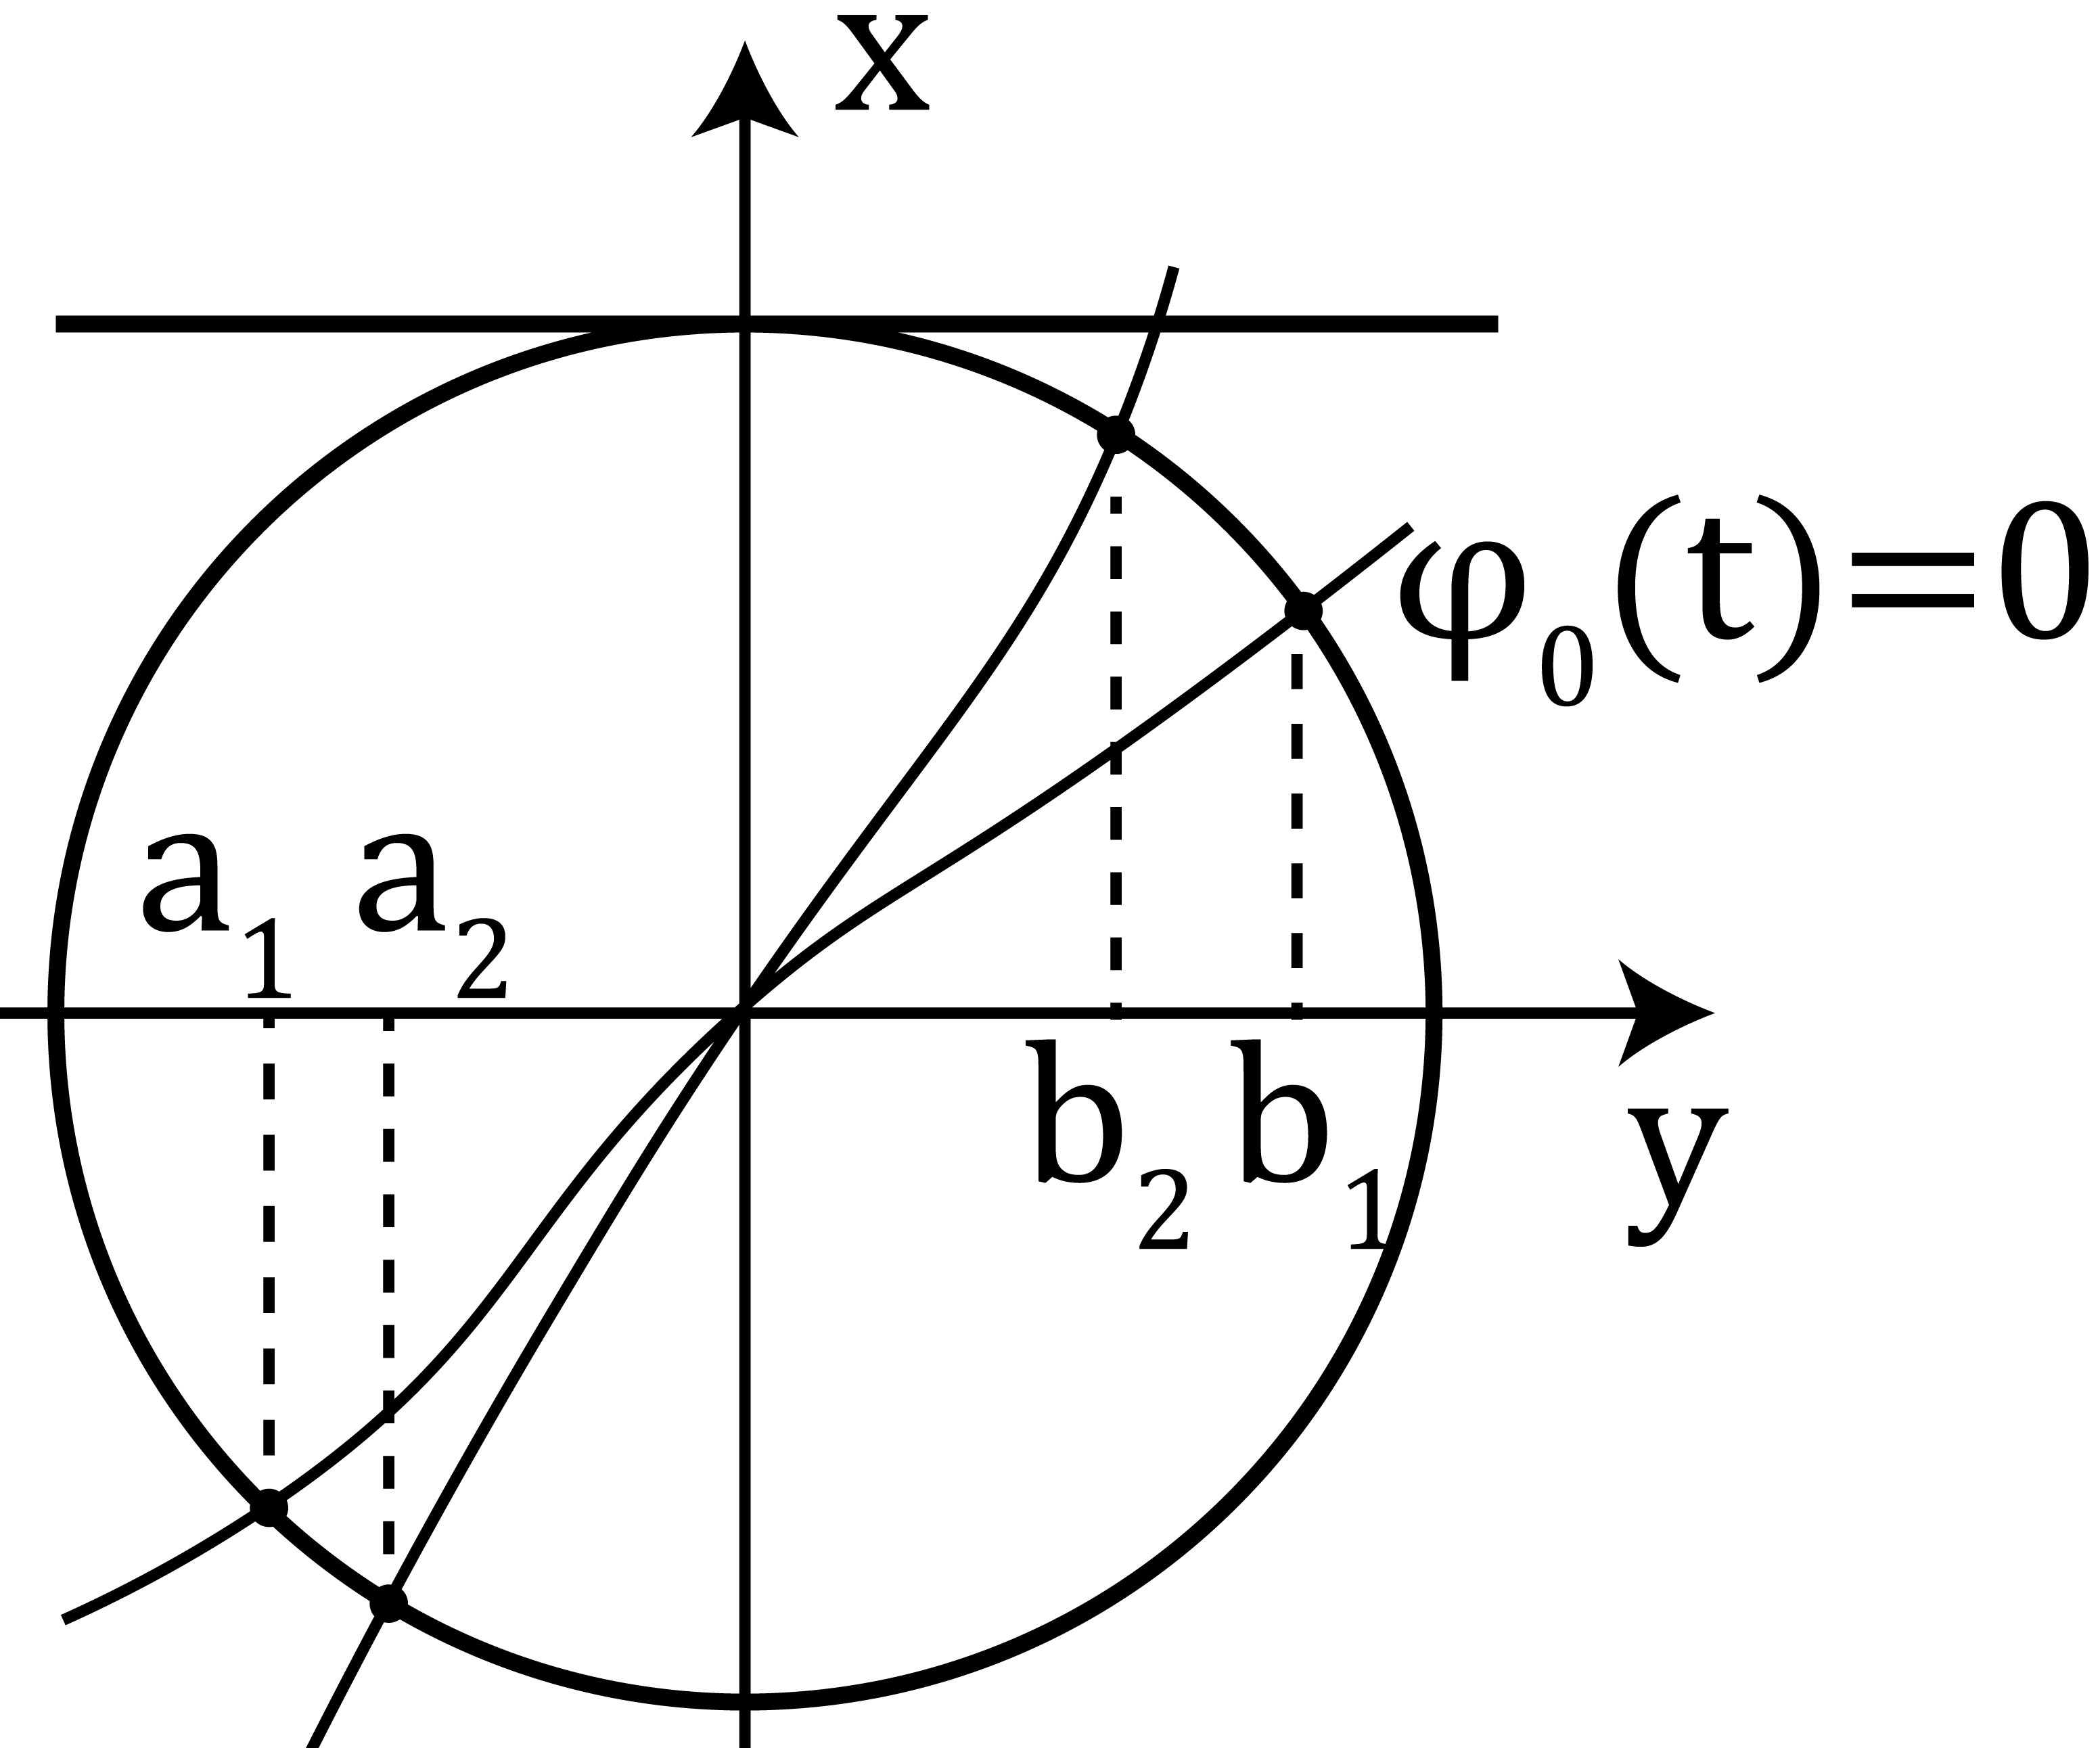
\includegraphics[width=4cm]{pics/8_1.png}
				    \centering
				\end{figure}

				\begin{enumerate}
						\item $(t_0, x_0) = (0, 0)$
							\[\varphi_0(t) = 0 \text{ - опред при } t \in [-1; 1]\]
							\[\varphi_1(t) \text{ - опред на } [a, b]\]
						\item $(t_0, x_0) = (0, 1) \qq \varphi_0(t) \equiv 1 $ опред при $t = 0$
				\end{enumerate}
		\end{Example}

		\begin{Theorem} [Пикара]
				\[(1), (2) \qq X \in C(D), \q D \text{ - замкн } \qq (D \subset \R^{n + 1} )\]
				\[X \in \Lip_x(D)\]
				\[\varphi_k(t) \text{ - опред на } [a, b] \q \forall k \in \{0\} \cup \N\]
				\[\Ra \q \varphi_k(t) \us{k \to +\infty}{\os{[a, b]}{ \rightrightarrows}}
				\varphi(t) \text{ и } \varphi(t) \text{ - реш З.К. } (1), (2)\]
		\end{Theorem}

		\begin{Proof}
				\[\text{Ряд } \q \varphi_0 + \sum_{k = 1}^\infty (\varphi_k - \varphi_{k - 1}) \q (6) \]
				\[\varphi_0 + (\varphi_1 - \varphi_0) + (\varphi_2 - \varphi_1) + ...\]
				\[S_k(t) = \varphi_k(t)\]
				\[\abs{\varphi_0(t)} = \abs{x_0}\]
				\[(7) \q \abs{\varphi_1(t) - \varphi_0(t)} =
					\abs{\int_{t_0}^t X(\tau, x_0)d\tau } \leq
				\abs{\int_{t_0}^t \abs{X(\tau,x_0)} d\tau } \leq\]
				\[\leq M\abs{t - t_0} \q \forall t \in [a, b]\]
				\[\exists M: \abs{X(t, x_0)} \leq M \q \forall t \in [a, b]\]
				\[\text{по усл : } \exists L > 0 : \forall (t, \overline{x}), (t,
				\ool{x}) \in D \qq \abs{X(t, \overline{x} - X(t, \overline{\overline{x}}))}\leq
				L\abs{\overline{x} - \overline{\overline{x}}} \q (8)\]
				\[\abs{\varphi_2(t) - \varphi_1(t)} = \abs{\int_{t_0}^t (X(\tau, \varphi_1(\tau)) -
				X(\tau, \varphi_0(\tau)))d\tau } \leq\]
				\[\leq \abs{\int_{t_0}^t \abs{X(\tau, \varphi_1(\tau)) - X(\tau, \varphi_0(\tau))}
				d\tau } \os{(8)}{\leq} L\abs{\int_{t_0}^t \abs{\varphi_1(\tau)  - \varphi_0} }d\tau
				\us{(7)}{\leq}\]
				\[\leq LM\abs{\int_{t_0}^t \abs{\tau - t_0 } d\tau} =
				M \cdot L \frac{\abs{t - t_0}^2}{2} = \frac{M}{L} \frac{(L\abs{t - t_0}^2)}{2} \q (9)\]
				\[\abs{\varphi_k(t) - \varphi_{k - 1}(t)} \leq \frac{M}{L}
				\frac{(L\abs{t - t_0})^k}{k!}\]
				\[\abs{\varphi_{k + 1}(t) - \varphi_k(t)}  \leq \abs{\int_{t_0}^t \abs{
				X(\tau, \varphi_k(\tau)) - X(\tau, \varphi_{k - 1}(\tau)) } d\tau} \os{(8)}{\leq}\]
				\[\leq L \abs{\int_{t_0}^t \abs{\varphi_k(\tau) - \varphi_{k - 1}(\tau)} d\tau }
				\os{(10)}{\leq} L\frac{M}{L} \abs{\int_{t_0}^t \frac{(L\abs{\tau - t_0}^k)}{k!}
				d\tau} = \]
				\[= \frac{M}{L} \frac{(L\abs{t - t_0})^{k  + 1} }{k!()}\]
				\[(11) \qq \abs{\varphi_k(t) - \varphi_{k - 1} } \leq \frac{M}{L}
				\frac{(L(b - a)^k)}{k!}\]
				\[(6) \qq \text{ мажоририруется рядом } \abs{x_0} + \sum_{k = 1}^\infty \frac{M}{L}
				\frac{(L(b - a))^k}{k!}\]
				\[\text{сх-ся к } \abs{x_0} + \frac{M}{L} (e^{L(b - a)} - 1) \]
				\[\Ra (6) \q \text{сх. абс. и равномерно на } [a, b] \Ra\]
				\[\Ra \varphi_k(t) \os{[a, b]}{\rightrightarrows} \varphi(t) \text{ и }
				(t, \varphi(t)) \in D \qq \forall t \in [a, b]\]
				\[(5) \qq \varphi_k(t) = x_0 + \int_{t_0}^t X(\tau, \varphi_{k - 1}(\tau) )d\tau \]
				\[\text{из } (8) : \abs{X(t, \varphi(t)) - X(t, \varphi_k(t))} \leq
				L\abs{\us{\rightrightarrows 0}{\varphi(t) - \varphi_k(t)}} \Ra\]
				\[\Ra X(t, \varphi_k(t)) \os{[a, b]}{\rightrightarrows} X(t, \varphi(t)) \Ra
				\text{в }(5) \text{ можно перейти к пределу}\]
				\[\Ra \varphi(t) = x_0 + \int_{t_0}^t X(\tau, \varphi(\tau))d\tau \text{, т.е.}\]
				\[\varphi(t) \text{ - решение (3) и реш. З.Коши (1),(2)}\]
		\end{Proof}

		\begin{Consequence}
				\[\varphi_0(t) \equiv x_0\]
				\[(5) \qq \varphi_k(t) = x_0 + \int_{t_0}^t
				X(\tau, \varphi_{k - 1}(\tau)) d\tau \]
				\[X \in C(\R^{n + 1} )\]
				\[X \in \Lip_x(\R^{n + 1} )\]
				\[\Ra \varphi_k(t) \text{ опред на } \R \text{ и } \varphi(t) \text{ опред
				на } \R\]
		\end{Consequence}

		\begin{Proof}
				\[\varphi_k(t) \text{ опред на } \R \q (\text{по } (5))\]
				\[\{h_k\}_{k = 1}^\infty, \q h_k \us{k \to +\infty}{\to } + \infty\]
				\[\forall [t_0 - h_k, t_0 + h_k] \text{ верна Т. Пеано, т.е}\]
				\[\varphi_k(t) \us{k \to +\infty}{\rightrightarrows} \varphi(t) \text{
				на отрезке } [t_0 - h_k, t_0 + h_k]\]
				\[\forall t - \text{ фикс } \exists h_k : t \in [t_0 - h_k, t_0 + h_k] \Ra
				\varphi(t) \text{ - опред } \forall t \in \R\]
		\end{Proof}

		\begin{Theorem}[1]
				\[\text{рассм. } (1), (2) \q D = \{(t, x) : \abs{t - t_0} \leq a,
				\abs{x - x_0} \leq b\} \qq a > 0 \q b > 0\]
				\[X \in C(D) \Ra \exists M: \abs{X(t, x)} \leq M \q \forall (t, x) \in D\]
				\[h = \min(a, \frac{b}{m}), \q X \in \Lip_x(D)\]

				\[\varphi_k(t) \text{ опред на } [t_0 - h, t_0 + h] \text{ и } \varphi_k(t)
				\os{[t_0 - h, t_0 + h]}{\us{k \to +\infty}{\rightrightarrows}} \varphi(t)
				\text{реш З. Коши (1), (2)}\]
		\end{Theorem}

		\begin{Proof}
				\[\varphi_0(t) \equiv x_0 \text{ - опр. на } [t_0 - h, t_0 + h]
				\qq \text{Пусть } \varphi_{k - 1} \text{ опред на } [t_0 - h, t_0 + h] \]
				\[\abs{\varphi_k(t) - x_0} \leq \abs{
						\int_{t_0}^t \us{\leq M}{\abs{X(\tau, \varphi_{k - 1} (\tau))} }
				d\tau} \leq M\abs{t - t_0} \leq Mh \leq b\]
				\[\Ra (t, \varphi_k(t)) \in D \text{, т.е } \varphi_k(t) \text{ - опред
				на } [t_0 - h, t_0 + h]\]
		\end{Proof}

		\begin{Consequence} [из теоремы 1]
				\[X \in C(G) \q X \in \Lip_x^{loc}(G) \qq G \text{ - обл. }
				G \subset \R^{n + 1}  \qq (t_0, x_0) \in G\]
				\[\Ra \exists h : \text{ при } t \in [t_0 - h, t_0 + h] \q
				\text{прибл. Пеано }  \varphi_k(t) \us{k \to +\infty}{\os{[t_0 - h, t_0 + h]}
				{\rightrightarrows}} \varphi(t) \text{ - реш. З.К } (1)(2)\]
		\end{Consequence}

		\begin{Proof}
				\[\forall (t_0, x_0) \in G \q \exists a > 0,\ b > 0 : \]
				\[D = \{(t, x) : \abs{t - t_0} \leq a, \q \abs{x - x_0} \leq b\} \subset G\]
				\[\text{и } X(t, x) \in \Lip_x(D)\]
		\end{Proof}

		\begin{remark}
				Т1 вместе со следствием - теорема о сущестовании решения
		\end{remark}

		%	\begin{remark}
		%			Локального условия Липшеца на всем пространсве не хватит для того,
		%			 чтобы решения были определены на всем $n$
		%	\end{remark}

		\begin{Remark}
				\[X \in C(\R^{n + 1}), \q X \in \Lip_x^{loc} (\R^{n + 1} ) \ \cancel{\Ra} \
				\varphi_k(t) \q\text{ опред на } \R\]
		\end{Remark}

		\begin{Proof}[Пример]
				\[\dot{x} = x^2 + 1 \qq \text{З.К } (0, 0)\]
				\[x^2 + 1 \in \Lip_{x}^{loc} (\R) \qq x^2 + 1 \cancel{\in } \Lip_x(\R)\]
				\[\frac{dx}{x^2 + 1} = dt\]
				\[\arctg x = t + c \qq \text{реш. З.К. } x = \tg t, \q t \in \left(
				-\frac{\pi}{2}, \frac{\pi}{2}\right)\]
		\end{Proof}

		\begin{Theorem} [2]
				\[X \in C(G) \qq X \in \Lip_x^{loc}(G) \qq (t_0, x_0) \in G \qq G \text{ - обл} \]
				\[\begin{matrix}
					x = \varphi(t)\\
					x = \psi(t)
				\end{matrix} \q \text{ реш З.Коши } (1), (2) \text{ опред на } <a,b>\]
				\[\Ra \varphi(t) \equiv \psi(t) \qq \forall t \in <a, b>\]
		\end{Theorem}
\end{lect}
\end{document}
